\chapter{Oplossing}
\label{oplossing}

Dit hoofdstuk belicht aan de hand van een case-study de praktische realisatie van een schaalbare tool voor software-analyse. De case-study in kwestie is een implementatie van GEMINI die werkt met een Cassandra i.p.v. SQLite databank. Achtereenvolgens komen een motivatie voor de keuze voor Cassandra, de nodige aanpassingen aan het dataschema van GEMINI, en de nodige aanpassingen aan de implementatie van de querying-functionaliteit van GEMINI aan bod.

\section{Keuze database}

\subsection{Vereisten}

Zoals beschreven in [\ref{gemini_beschrijving}] bewaart GEMINI de data over genetische varianten en proefpersonen in enkele zeer grote tabellen. Een eerste vereiste voor een database is dus om deze tabulaire data goed te kunnen voorstellen en beheren. Omdat de nadruk van dit onderzoek specifiek ligt op het schaalbaar maken van de applicatie, gebeurt dit bij voorkeur d.m.v. automatische verspreiding over verschillende nodes in een cluster.\\
Omdat GEMINI meerdere processoren of zels computers kan gebruiken bij het inladen van de gegevens uit VCF-bestanden, is goede concurrency controle en hoge schrijf-throughput eveneens belangrijk. Na het inladen van de VCF bestanden voert GEMINI enkel nog lees-queries uit, dus zijn de belangrijkste verdere vereisten voor een database hoge lees-throughput, goede query-mogelijkheden en indexeringsmechanismes.
\\Ten laatste is een Python-API ook nuttig, gezien GEMINI in Python ge\"implementeerd is.

\subsection{Keuze}

De uiteindelijke keuze voor een databank viel op Apache Cassandra. Van de systemen besproken in [\ref{nosql_survey}] heeft Cassandra veruit de meest interessante architectuur qua schaalbaarheid en bovendien leent het columnaire model zich goed tot het modelleren van de tabellen in de oorspronkelijke versie van GEMINI. Vergeleken met het andere columnaire systeem, HBase, heeft Cassandra uitgebreidere query-mogelijkheden. Vergeleken met MongoDB, dat sterker staat op het gebied van querying en indexing heeft Cassandra het voordeel dat het flexibeler is voor concurrent schrijven naar de databank. Bovendien blijkt uit eerdere experimenten met MongoDB binnen het lab dat MongoDB niet space-effici\"ent BSON-documenten kan uitbreiden {\color{red} TODO}. %TODO
In het geval van een incrementele versie van GEMINI, waar na verloop van tijd genoominformatie van extra proefpersonen ingeladen moet worden, leidt dit tot fragmentatie. Cassandra daarentegen kan eenvoudig het schema van tabellen aanpassen en naar behoefte extra kolommen en rijen toevoegen.\\
Zoals later uitgebreid aan bod komt, heeft Cassandra ook nadelen. Vooral de eerder beperkte query-capaciteiten bemoeilijken het implementeren van de uitgebreide ad-hoc queryfunctionaliteiten van GEMINI.

\section{Conceptueel ontwerp}

\subsection{Dataschema}

\label{cassandra_datamodel}

Het datamodel van Apache Cassandra vertoont enkele sterke verschillen met het relationele datamodel. Dit vereist enkele grondige aanpassingen aan het database schema van GEMINI. In deze sectie komen de belangrijkste eigenschappen van Cassandra aan bod, hun gevolgen voor de belangrijkste database-functionaliteiten, en een conceptuele schets van benodigde aanpassingen aan het onderliggende dataschema van GEMINI.

\subsubsection{Datamodel Cassandra}

Zoals eerder vermeld bewaart Cassandra de cellen in een tabel als een 2 dimensionele map van enerzijds een per rij gedefinieerde primary key, en de naam van een kolom. De inhoud van cellen die niet in de primary key van een rij liggen, heeft voor Cassandra geen enkele betekenis.\\
Die primary key bestaat uit 2 delen: het eerste is de partition key, deze bestaat uit minstens 1 kolom en de waarde hiervan die via het consistent-hashing mechanisme bepaalt op welke partitie in het cluster de rij terechtkomt. Het tweede, optionele, deel is de clustering key, en bepaalt in welke volgorde rijen met dezelfde partition key op 1 node bewaard worden. Dit is standaard in oplopende volgorde.\\

%TODO ALLOW FILTERING
Omdat het inspecteren van cellen indruist tegen de principes van Cassandra, zijn de query-mogelijkheden eerder beperkt: zonder het defini\"eren van indices is het in \texttt{WHERE}-clausules enkel mogelijk beperkingen op te leggen aan kolommen in de primary key, en dan nog zo dat de bedoelde rijen binnen 1 partitie liggen, en opeenvolgend opgeslagen zijn. Daarom moet er een gelijkheidsbeperking opgelegd worden aan de volledige partition key, en mogen er zowel gelijk- als ongelijkheidsbeperkingen opgelegd worden aan de kolommen in de clustering key, maar enkel op voorwaarde dat de voorgaande kolom in de clustering key ook met een gelijkheidsbeperking gespecifieerd is. Op deze manier kan Cassandra queries zeer snel uitvoeren door ze a.d.h.v. de hash van de partition key naar een juiste node te routeren, en vervolgens via de overige opgegeven kolommen de locatie van de juiste rijen te berekenen (die omwille van de clustering allemaal opelkaar volgend opgeslagen zijn). Dit gebeurt zonder de waarden van individuele cellen te bekijken, maar dus enkel door het berekenen van een simpele hashfunctie. Range-queries zijn dus enkel mogelijk op kolommen in de clustering key en het is niet mogelijk \texttt{!=}-beperkingen te gebruiken in \texttt{WHERE}-clausules. Bovendien laat Cassandra enkel toe beperkingen met elkaar te combineren via conjuncties, dus niet via \texttt{OR}- of \texttt{NOT}-operatoren. Een uitzondering op dit laatste is de \texttt{IN}-operator: op deze manier kan de gebruiker meegeven in welke set van waarden een bepaalde kolom moet liggen, maar dit is ook enkel mogelijk op de laatste kolom in de partition key of de laatste kolom in de clustering key (maar weer op voorwaarde dat de voorgaande kolommen reeds beperkt zijn).\\
Cassandra laat toe om indices op kolommen te defini\"eren, maar deze zijn niet bijzonder nuttig. Ze laten enkel gelijkheidsbeperkingen toe (dus geen range-queries) en bovendien raadt Datastax het gebruik van indices op kolommen met zowel een zeer lage als een zeer hoge kardinaliteit af, dit omdat in het eerste geval de index tabel zal bestaan uit zeer weinig zeer lange rijen voor elk van de ge\"indexeerde waarden en in het tweede geval Cassandra bij een query op de ge\"indexeerde kolom door zeer veel verscheidene waarden zal moeten zoeken om een klein aantal resultaten te vinden \cite{when_to_use_index}.

\subsubsection{Databaseschema GEMINI}

Zoals blijkt uit bovenstaande beschrijving van het datamodel van Cassandra, leent het systeem zich niet goed tot ad-hoc querying: het is niet mogelijk op een performante manier zomaar aan willekeurige kolommen in een tabel voorwaarden op te leggen en deze voorwaarden met elkaar te combineren. Dit betekent dat bij het ontwerpen van het database schema al rekening gehouden moet worden met de queries die achteraf op de data mogelijk moeten zijn. Omdat het soort queries dat een tabel ondersteunt sterk samenhangt met de keuze van de primary key van de tabel en GEMINI meerdere, uiteenlopende soorten queries op elke tabel vereist, zal dit onvermijdelijk leiden tot duplicatie van data.\\\\
In deze paragraaf komen meerdere schematische voorstellingen van databanktabellen voor. Om de leesbaarheid te verhogen, zijn hierin de namen van kolommen uit de partition key steeds in het {\color{green} groen} en van kolommen uit de clustering key in het {\color{red} rood} weergegeven.

\paragraph{\texttt{variants}-tabel vs. genotype-informatie}

Het belangrijkste vraagstuk is hoe de genotype-kolommen uit het oorspronkelijke relationele model in Cassandra op te slaan. Hier zijn enkele opties voor:

\begin{itemize}

\item \textbf{Collection columns} Cassandra biedt zogenaamde collection types, zoals sets, lists of maps. Dit is vergelijkbaar met de bestaande implementatie in SQLite (buiten dat ze in Cassandra niet als binary blobs bewaard worden). Het nadeel is echter dat deze collections niet meer dan 65536 ($2^{16}$) entries kunnen bevatten, wat het hele nut van de migratie naar Cassandra zou ondermijnen.

\item \textbf{Super-\texttt{variants}-tabel} Een andere mogelijkheid is de \texttt{variants}-tabel uit te breiden met een kolom voor elke genotype-eigenschap van elke sample. Deze aanpak heeft als voornaamste voordeel dat de kolommen met genotype-eigenschappen van specifieke samples zonder omwegen uit de \texttt{variants}-tabel gehaald kunnen worden. Dit is vooral van belang voor de in (\ref{gemini_beschrijving}) beschreven sample-filters. Bovendien kan Cassandra tot 2 miljard cellen opslaan op 1 partitie, dus vormt het grote aantal kolommen dat dit model met zich meebrengt, geen probleem.\\
Het nadeel is echter dat het onmogelijk is ad-hoc queries te defini\"eren op genotypes van willekeurige eigenschappen zonder het gebruik van secundaire indices. Elke query die in een \texttt{WHERE}-clausule andere kolommen of samples betrekt, vereist om de hierboven beschreven redenen een andere keuze van de primary key om effici\"ent de juiste rijen te kunnen opzoeken.

\begin{table}[!htbp]
\begin{tabular}{@{}|l|l|l|l|l|l|l|l|l|l|@{}}
\toprule
\color{green} variant\_id & ref & alt & \ldots & gt\_type\_alex & gt\_type\_john & \ldots & gt\_depth\_alex & gt\_depth\_john & \ldots \\ \bottomrule
\end{tabular}
\end{table}

\item \textbf{\texttt{genotype}-tabellen} Een derde optie is een \texttt{variants}-tabel zonder genotype-informatie, gecombineerd met een tabel voor elke eigenschap van de genotypes van de samples, met een rij voor elke \texttt{(variant, sample)}. Bijvoorbeeld:\\

\begin{itemize}

\item Een \texttt{variants\_by\_samples\_gt}-tabel met als primary key \texttt{((sample\_name, gt\_type), (variant\_id))}. De primary key is zo gekozen dat alle variants waarvoor een sample eenzelfde genotype heeft, bij elkaar op 1 node liggen, zodat deze gemakkelijk opgevraagd kunnen worden. Hetzelfde was mogelijk geweest met enkel \texttt{sample\_name} als partition key, maar met de bovenstaande, granulairdere partition key zijn de variants beter over het cluster verspreid. Bovendien houdt het vanuit een semantisch oogpunt geen steek range queries uit te voeren op de \texttt{gt\_type}-kolom, dus moet deze niet per se in de clustering key staan. De \texttt{variant\_id}-kolom ten slotte maakt enkel deel uit van de primary key om deze uniek te maken voor elk tupel \texttt{(variant, sample, genotype)}.\\

\begin{table}[!htbp]
\begin{tabular}{@{}|l|l|l|@{}}
\toprule
\color{green} sample\_name & \color{green} genotype & \color{red} variant\_id \\ \bottomrule
\end{tabular}\\
\end{table}

\item Een \texttt{variants\_by\_samples\_gt\_depth}-tabel met als primary key \texttt{((sample\_name), (gt\_depth, variant\_id))}. Omdat range queries op de \texttt{gt\_depth}-kolom wel een vereiste zijn, moeten alle variants voor eenzelfde sample volgens gt\_depth geclusterd, en dus gerangschikt staan. Vandaar dat de \texttt{gt\_depth}-kolom in dit geval in de clustering key, en niet in de partition key staat. Voor de rest is de keuze van de primary key volledig analoog met die in de \texttt{variants\_by\_samples\_gt}-tabel.

\begin{table}[!htbp]
\begin{tabular}{@{}|l|l|l|@{}}
\toprule
\color{green} sample\_name & \color{red} gt\_depth & \color{red} variant\_id \\ \bottomrule
\end{tabular}
\end{table}

\item Vergelijkbare tabellen voor de overige genotype-eigenschappen.

\end{itemize}

Het grote voordeel van deze aanpak is dat het, dankzij de keuze van de primary key, zeer eenvoudig is variants op te vragen waarvoor het genotype van \'e\'en sample aan specifieke gelijkheids- of ongelijkheidsvoorwaarden voldoet. Het nadeel van dit schema is drieledig: ten eerste scheidt het de informatie over de genotypes van samples van de andere informatie over de variants. Dit betekent dat, om deze samen weer te geven, een \texttt{JOIN} van de \texttt{variants}-tabel met een \texttt{genotype}-tabel nodig is, en Cassandra biedt zoals geweten geen \texttt{JOIN}. Ten tweede is het onmogelijk om met een sample-filter voor meerdere samples de genotypes tegelijkertijd op te vragen, en ten laatste is het onmogelijk in een query voorwaarden op te leggen aan de genotypes van meerdere samples.

\end{itemize}

De uiteindelijke keuze is gevallen op een combinatie van de tweede en derde optie. Dit om de volledige oorspronkelijke functionaliteit van GEMINI te kunnen bieden: enerzijds het opvragen van de genotype-informatie van willekeurige samples door middel van de sample-filters, en anderzijds het query'en van de \texttt{variants}-tabel met, dankzij gt-filters en -wildcards, beperkingen op de genotypes van specifiek gekozen samples. Zoals hierboven beschreven is dit laatste niet voor de hand liggend, en zal door het ontbreken van \texttt{JOIN}s en de layout van de \texttt{genotype}-tabellen het combineren van beperkingen op de genotypes van meerdere samples nog extra aanpassingen vergen. Hier gaan secties \ref{gemini_query_concept} en \ref{gemini_query_impl} dieper op in.

\paragraph{\texttt{variants-, samples-}tabel vs. arbitraire queries}

Een tweede belangrijke vraagstuk is hoe de \texttt{variants-} en \texttt{samples-}tabellen zo te ontwerpen dat ze ook op andere, arbitraire kolommen effici\"ent doorzoekbaar zijn.\\
Om queries op kolommen te ondersteunen die logisch gezien enkel met gelijkheden beperkt zullen worden, zoals \texttt{chrom} of respectievelijk \texttt{sex}, zou het in theorie volstaan op deze kolommen een secundaire index te defini\"eren. Dit is eenvoudig bij de creatie van de tabel, veroorzaakt geen duplicatie van data en is zeer rechttoe-rechtaan bij het query'en, maar heeft zoals hierboven vermeld onvoorspelbare performantie afhankelijk van de kardinaliteit van de kolommen. Bovendien werkt dit mechanisme niet voor kolommen die vaker met ongelijkheidsbeperkingen gequeried zullen worden, zoals \texttt{depth}, \texttt{start}, of in het geval van de \texttt{samples}-tabel (hypothetisch, deze tabellen zitten niet standaard in GEMINI) leeftijd of generatie.\\

Een aanpak die in beide gevallen op een voorspelbare en betrouwbare manier werkt, is om net als voor de genotype-informatie extra tabellen te defini\"eren, met een specifiek gekozen primary key die de gewenste query mogelijk maakt. Deze oplossing zorgt natuurlijk voor veel gedupliceerde data, maar heeft als voordeel dat ze \'e\'en coherente en performante aanpak van het probleem mogelijk maakt. Bij het opstellen van deze tabellen moet goed overwogen worden welke vaakgebruikte queries een eigen tabel vereisen en verdienen. Minder frequente, uitgebreidere queries, kunnen mits een goede keuze van de basistabellen immers gesplitst worden in subqueries op deze basistabellen. Hetzelfde mechanisme dat voor de gt-filters en -wildcards uitgebreide queries zal uitvoeren is ook hier van toepassing. Dit zal natuurlijk minder effici\"ent zijn dan een aangepaste tabel voor de uitgebreide, originele query, maar laat toe de data-duplicatie enigszins binnen de perken te houden. Voorbeelden van zulke basistabellen zijn:

\begin{itemize}
\item Een \texttt{variants\_by\_chrom\_start}-tabel, die het eenvoudig maakt alle varianten op te zoeken die op een bepaald chromosoom binnen een range van startposities liggen. De primary key is in dit geval: \texttt{((chrom), (start, variant\_id))}. 

\begin{table}[!htbp]
\begin{tabular}{@{}|l|l|l|@{}}
\toprule
\color{green} chrom & \color{red} start & \color{red} variant\_id \\ \bottomrule
\end{tabular}
\end{table}

\item Een \texttt{variants\_by\_gene}-tabel, die het eenvoudig maakt alle varianten binnen \'e\'en gen op te zoeken. De primary key is in dit geval: \texttt{((gene), (variant\_id))}.

\begin{table}[!htbp]
\begin{tabular}{@{}|l|l|@{}}
\toprule
\color{green} gene & \color{red} variant\_id \\ \bottomrule
\end{tabular}
\end{table}

\item Een \texttt{samples\_by\_sex}-tabel, die het eenvoudig maakt alle samples van een bepaald geslacht op te vragen. De primary key is in dit geval: \texttt{((sex), (sample\_name))}.

\begin{table}[!htbp]
\begin{tabular}{@{}|l|l|@{}}
\toprule
\color{green} sex & \color{red} sample\_name \\ \bottomrule
\end{tabular}
\end{table}
\end{itemize}

Ten slotte is het ook nog interessant een feature aan de gebruikersinterface van GEMINI toe te voegen waarmee de gebruiker zelf nieuwe basistabellen kan defini\"eren wanneer hij dit nodig acht.

\paragraph{\texttt{JOIN}s}

Zoals eerder aangehaald, biedt Cassandra geen \texttt{JOIN}s in de bijhorende querytaal CQL. In de plaats moedigt Cassandra het \textit{materializeren} van \texttt{JOIN}s aan, namelijk het samen bewaren van gegevens die samen opgevraagd zullen worden. Dit leidt tot de denormalizatie t.o.v. relationele dataschema's, die ontworpen zijn om zo opslageffici\"ent mogelijk alle data voor te stellen en zwaar inzetten op \texttt{JOIN}s om gegevens uit verschillende tabellen met elkaar te combineren.\\
GEMINI biedt de gebruiker ook de optie verschillende tabellen samen te doorzoeken m.b.v. \texttt{JOIN}s. Enkele voorbeelden zijn:

\lstinputlisting[language=SQL]{vb_SQL_queries/joins.txt}

Dankzij het hierboven beschreven query-mechanisme is het echter niet nodig alle tabellen die met elkaar gejoind zouden kunnen worden, ook effectief samen op te slaan in 1 tabel. Door weeral juist gekozen hulptabellen te defini\"eren, kunnen het reeds uitgelegde datamodel en query-mechanisme ook hier van dienst zijn.\\
Om de eerste van de twee queries uit bovenstaand voorbeeld uit te voeren, is dan bijvoorbeeld een tabel nodig die het mogelijk maakt alle variants met een bepaalde \texttt{impact\_severity} op te vragen (bvb. \texttt{variants\_by\_impact\_severity}), en een tweede tabel die toelaat alle genen uit \texttt{gene\_detailed} op te vragen voor een bepaalde waarde van de \texttt{gene} en \texttt{chrom} kolommen (bvb. \texttt{gene\_detailed\_by\_gene\_chrom}). De gewenste variants kunnen opgehaald worden uit de \texttt{variants\_by\_impact\_severity}-tabel en vervolgens kunnen via de \texttt{gene\_detailed\_by\_gene\_chrom} alle gewenste kolommen uit de \texttt{variants}- en \texttt{gene\_detailed}-tabellen geselecteerd worden. Een analoge redenering gaat op voor de tweede voorbeeldquery en bij uitbreiding ook voor de andere voor GEMINI relevante \texttt{JOIN}s \cite{gemini_joins}.

\subsection{\texttt{gemini load}}

Het inladen van de genoomdata in de GEMINI-databank is conceptueel erg eenvoudig: elke lijn uit een VCF-file komt overeen met een variant en dus een rij in de \texttt{variants}-tabel (en de bijhorende hulptabellen), elke lijn in een PED-file met een sample en dus een rij in de \texttt{samples}-tabel (en de bijhorende hulptabellen). Het inladen kan bovendien versneld worden door de text-input te verdelen over verschillende cores en deze in parallel de data te laten invoeren.

\subsection{\texttt{gemini query}}
\label{gemini_query_concept}
Het uitvoeren van de gewoonlijke GEMINI-queries tegen een Cassandra-databank vergt enkele ingrijpende aanpassingen ten opzichte van de SQLite-versie van Cassandra. Het doel is natuurlijk deze aanpassingen zoveel mogelijk te verbergen voor de gebruiker, wat ook in grote mate gelukt is. In deze sectie komt achtereenvolgens aan bod hoe ingewikkelde queries gesplitst worden in eenvoudige subqueries, hoe de resultaten hiervan vervolgens gecombineerd worden en wat dit betekent voor de meest geavanceerde feature van GEMINI, namelijk de genotype-filter wildcards.

\subsubsection{Splitsing in subqueries}

Zoals beschreven in \ref{cassandra_datamodel}, kan Cassandra enkel effici\"ent queries uitvoeren die beperkingen opleggen aan de kolommen in de primary key van een tabel, en dit ook slechts onder bepaalde voorwaarden. Bovendien is de enige logische operator die Cassandra ondersteunt om beperkingen te combineren, de conjunctie.\\
Om arbitraire queries en \texttt{WHERE}-clausules te ondersteunen, kan GEMINI niet zoals in de SQLite-versie de \texttt{WHERE}-clausule zomaar onveranderd aan Cassandra doorgeven. Beschouw, ter illustratie, volgende query:\\\\
\texttt{SELECT chrom, start, subtype FROM variants WHERE chrom = 'chromX' \\AND start > 5600 AND gene = 'gene\_A'}.\\\\
Deze query valt uiteen in 2 subqueries: een eerste om uit de \texttt{variants\_by\_chrom\_start}-tabel alle variants op te vragen die voldoen aan de voorwaarde \texttt{chrom = 'chromX' AND start > 5600} en een tweede om uit de \texttt{variants\_by\_gene}-tabel alle variants die voldoen aan \texttt{gene = 'gene\_A'} op te vragen.\\

\subsubsection{Combineren subqueries}
\label{comb_subq_concept}
De subqueries zullen elk een verzameling rijen als resultaat opleveren. Het is dan zaak deze verzamelingen met set-operaties te combineren tot de finale verzameling rijen die aan de query voldoen. De nodige set-operatie hangt af van de oorspronkelijke query. Zo zal het eindresultaat van een conjunctie van subqueries de doorsnede van de resultaatverzamelingen van de subqueries zijn. In het geval van een disjunctie is dit de unie van de resultaatverzamelingen, en in het geval van een negatie van een subquery is dit het verschil tussen de oorspronkelijke verzameling (voor de query) en de resultaatverzameling van de query. Om bijvoorbeeld alle varianten te vinden die niet op een bepaald gen x liggen, moet het verschil bepaald worden tussen de verzameling van alle varianten en de verzameling van alle varianten die op gen x liggen. Tabel \ref{combineren_subqueries} vat dit samen voor 2 subqueries $p$ en $r$, hun respectievelijke resultaatverzamelingen $res(p)$ en $res(r)$ en een initi\"ele verzameling rijen $I$.

\begin{table}[h]
\centering
\begin{tabular}{|l|l|}
\hline
\textbf{Query} & \textbf{Resultaat}    \\ \hline
$p$ \texttt{AND} $r$ & $res(p) \cap res(r)$   \\ \hline
$p$ \texttt{OR} $r$ & $res(p) \cup res(r)$    \\ \hline
\texttt{NOT} $p$  & $I \setminus res(p)$ \\ \hline
\end{tabular}
\caption{De verschillende manieren om subqueries met elkaar te combineren.}
\label{combineren_subqueries}
\end{table}

\subsubsection{Genotype-filter wildcards}

Ter herinnering, de structuur van een genotype-filter wildcard:\\\\
\texttt{(genotype\_column).(sample\_wildcard).(gt\_wildcard\_rule).(rule\_enforcement)}\\\\
Het uitvoeren en evalueren van deze wildcards is conceptueel niet erg ingewikkeld: het volstaat de \texttt{sample\_wildcard} te evalueren en vervolgens voor elk van de resulterende samples een subquery op te stellen op de voor \texttt{genotype\_column} relevante hulptabel van de \texttt{variants}-tabel. Hoe deze subqueries met elkaar gecombineerd moeten worden, hangt af van de gegeven \texttt{rule\_enforcement}:

\begin{itemize}
\item Een \texttt{all}-wildcard leidt tot de conjunctie van alle subqueries.
\item Een \texttt{any}-wildcard leidt tot de disjunctie van alle subqueries.
\item Een \texttt{none}-wildcard leidt tot de conjunctie van de negaties van alle subqueries.
\item \texttt{count}-wildcards vallen niet zomaar met set-algebra te evalueren: bij het combineren van de resultaten van alle subqueries moet voor elke variant geteld worden in de resultaatverzameling van hoeveel subqueries hij voorkomt. Nadien kan GEMINI eenvoudig op basis van deze tellingen de varianten bepalen die aan de \texttt{count}-regel voldoen.
\end{itemize}

Dit betekent dat weer veel werk van de databank naar GEMINI zelf verschuift. Een mogelijke manier om dit leed te verzachten is, gezien de goede concurrency-eigenschappen van NoSQL-systemen als Cassandra, om de subqueries in parallel te evalueren in plaats van sequentieel.

\section{Implementatie}
\subsection{\texttt{gemini load}}
Het inladen van genoomdata in GEMINI gebeurt in twee stappen. De reden voor deze opsplitsing is dat een klein deel van het inladen en initialiseren van de databank niet parallel op meerdere processoren kan verlopen. \\In de eerste en kleinste van de twee, initialiseert GEMINI de databank, maakt de nodige tabellen aan en laadt de samples-informatie in. GEMINI haalt de namen van de samples uit de VCF-file, en vult deze aan met informatie uit de PED-file. Indien er geen PED-file voorhanden is, initialiseert GEMINI de \texttt{samples}-tabel met default-waarden voor de kolommen zoals \texttt{sex} en \texttt{phenotype}. Meteen worden ook de extra, aan de \texttt{samples}-tabel verbonden tabellen zoals \texttt{samples\_by\_sex} en \texttt{samples\_by\_phenotype} aangemaakt en gevuld. Ook de \texttt{resources-, gene\_detailed-, gene\_summary-} en \texttt{version-}tabellen worden in deze fase gevuld. Dit omdat de pedigree-files en de bestanden met data over de genen niet effici\"ent opgesplitst kunnen worden. Bovendien is de duur van het inladen van de \texttt{samples}-tabel zelfs bij 10000'en samples verwaarloosbaar tegenover het inladen en annoteren van de \texttt{variants}-tabel.\\
In de tweede fase gebeurt het leeuwendeel van het werk: het inladen van de variants-informatie uit de (verplicht meegegeven) VCF-file. Dankzij de bgzip \cite{bgzip} en grabix \cite{grabix} tools kan GEMINI effici\"ent VCF-bestanden in blokken opsplitsen, comprimeren, hierop een index defini\"eren en vervolgens daarmee verderwerken. Zo kan GEMINI eenvoudig het inladen van de variants, die elk \'e\'en lijn in de VCF-file in beslag nemen, gemakkelijk over meerdere cores verdelen. Het is ook in deze fase dat GEMINI de aan de \texttt{variants}-tabel verwante tabellen zoals \texttt{variants\_by\_samples\_gt\_type}, \texttt{variants\_by\_samples\_gt\_depth} en \texttt{variants\_by\_chrom\_start} opvult. Alle cores of nodes in het cluster, voeren rechtstreeks rijen in in \'e\'en en dezelfde tabel in de Cassandra-databank. Omdat Cassandra atomiciteit binnen rijen garandeert en alle workers strikt disjuncte sets van variants invoeren in het systeem, is er geen enkel risico op conflicten.\\\\
De grote winst ten opzichte van de SQLite-implementatie van GEMINI is dat in het parallelle gedeelte, alle workers naar dezelfde databank kunnen schrijven. In de SQLite-versie van GEMINI schrijven alle workers naar een aparte SQLite-database, die vervolgens in een kostelijke operatie nog allemaal samengevoegd moeten worden tot \'e\'en grote SQLite-databank. Deze stap (het \texttt{gemini merge}-commando) kan de Cassandra-implementatie volledig overslaan. Een ander opzicht waarin de Cassandra-implementatie effici\"enter is dan de SQLite-versie, is dat in SQLite voor elke variant de genotype-kolommen nog tot binary blobs gecomprimeerd worden. In Cassandra is dit, dankzij de keuze van het databaseschema, niet nodig.

\subsection{\texttt{gemini query}}
\label{gemini_query_impl}

\subsubsection{Splitsing in subqueries}

Om beslissingen zoals in het voorbeeld dynamisch te kunnen maken, is het nodig de \texttt{WHERE}-clausule te inspecteren en hieruit de benodigde hulptabellen voor de subqueries te identificeren. Om dit proces te vereenvoudigen, heb ik ervoor gekozen de query syntax licht aan te passen: beperkingen die binnen 1 hulptabel liggen, kunnen nog steeds met elkaar gecombineerd worden met het \texttt{AND}-keyword, maar beperkingen die niet binnen eenzelfde hulptabel liggen, moeten met de \texttt{\&\&, ||} of \texttt{NOT}-operatoren van elkaar gescheiden worden. Zo kan GEMINI bij het parsen van de \texttt{WHERE}-clausule deze onmiddellijk opsplitsen in subqueries en voor elk van deze subqueries de nodige hulptabel bepalen. Beschouw wederom volgende query:\\\\
\texttt{SELECT chrom, start, subtype FROM variants WHERE chrom = 'chromX' \\AND start > 5600 AND gene = 'gene\_A'}.\\\\
In de aangepaste syntax wordt dit:\\\\
\texttt{SELECT chrom, start, subtype FROM variants WHERE chrom = 'chromX' \\AND start > 5600 \&\& gene = 'gene\_A'}.\\

Dit vereist uiteraard dat de gebruiker op de hoogte is van welke hulptabellen er bestaan. Gebruikers moeten sowieso weten op welke kolommen ze queries kunnen defini\"eren, en bijgevolg ook welke hulptabellen er bestaan. Bovendien bestaat het doelpubliek van GEMINI uit onderzoekers die het programma intensief gebruiken en dus voldoende gelegenheden hebben om dergelijke aanpassingen snel onder de knie te krijgen.\\
%TODO
Een andere optie is de syntax onveranderd te laten en uit de in de \texttt{WHERE}-clausule vermelde kolommen benodigde hulptabellen af te leiden. Deze aanpak heeft als voordeel dat de interface naar de gebruiker niet verandert, maar gezien nog steeds enkel queries mogelijk zijn op kolommen uit de hoofdtabel waarvoor hulptabellen bestaan, is achterwaartse compatibiliteit hiermee nog niet verzekerd. Daarbovenop levert deze aanpak ook nieuwe problemen op, zoals: wat met kolommen die in meerdere hulptabellen voorkomen, welke combinatie van tabellen wordt er dan best geselecteerd? Dergelijke vraagstukken neigen naar query-optimization en vallen buiten het ... {\color{red} TODO} Daarom verkoos ik de macht bij de gebruiker te leggen en te vertrouwen op diens oordeelkundigheid.\\\\
De gebruiker dient er ook rekening mee te houden dat Cassandra range-queries enkel onder strikte voorwaarden ondersteunt, namelijk (zoals eerder uitgelegd) enkel op clustering columns en enkel wanneer de voorgaande kolommen in de clustering key met gelijkheden beperkt zijn. Dit impliceert dat er slechts een range query op 1 kolom in een tabel mogelijk is. Daarnaast biedt Cassandra ook geen \texttt{!=}-operator. Dit euvel valt te verhelpen door een \texttt{!=}-clausule om te zetten naar een gelijkheidsbeperking en deze vervolgens te negeren. Een clausule als \texttt{phenotype != 2} wordt dan \texttt{NOT (phenotype = 2)}. Dit vereist dat de \texttt{!=}-clausule een aparte subquery vormt.\\

Het uiteindelijke algoritme om de geschikte hulptabel te selecteren op basis van de kolommen en gebruikte operatoren in een subquery, gebruikt de metadata van het Cassandra-cluster om alle hulptabellen voor een gegeven hoofdtabel op te vragen, en vervolgens aan de hand van de kolommen in de primary keys van de kandidaat-hulptabellen de geschikte eruit te kiezen.\\

GEMINI encapsuleert de subqueries in \texttt{query\_expression}s: een set Python-klassen die, ge\"inspireerd door algebra\"ische datatypes uit functionele talen zoals Haskell, alle mogelijke GEMINI-queries kunnen voorstellen. Deze bevatten alle informatie die GEMINI nodig heeft om de queries te evalueren. De \texttt{Basic\_expression} stelt een eenvoudige query op een Cassandra-tabel voor. Tijdens het parsen van de \texttt{WHERE}-clausule zal GEMINI de subqueries inkapselen in \texttt{Basic\_expressions} en deze, afhankelijk van de gehele query, nesten in \texttt{AND\_}-, \texttt{OR\_}- of/en \texttt{NOT\_expression}s. De \texttt{GT\_wildcard\_expression} stelt op een effici\"ente manier genotype-filter wildcards voor (zie \ref{gt_wildcards}). De volgende paragraaf bespreekt in detail de aangeboden \texttt{evaluate}- en \texttt{can\_prune}-functies.

\begin{figure}[h]
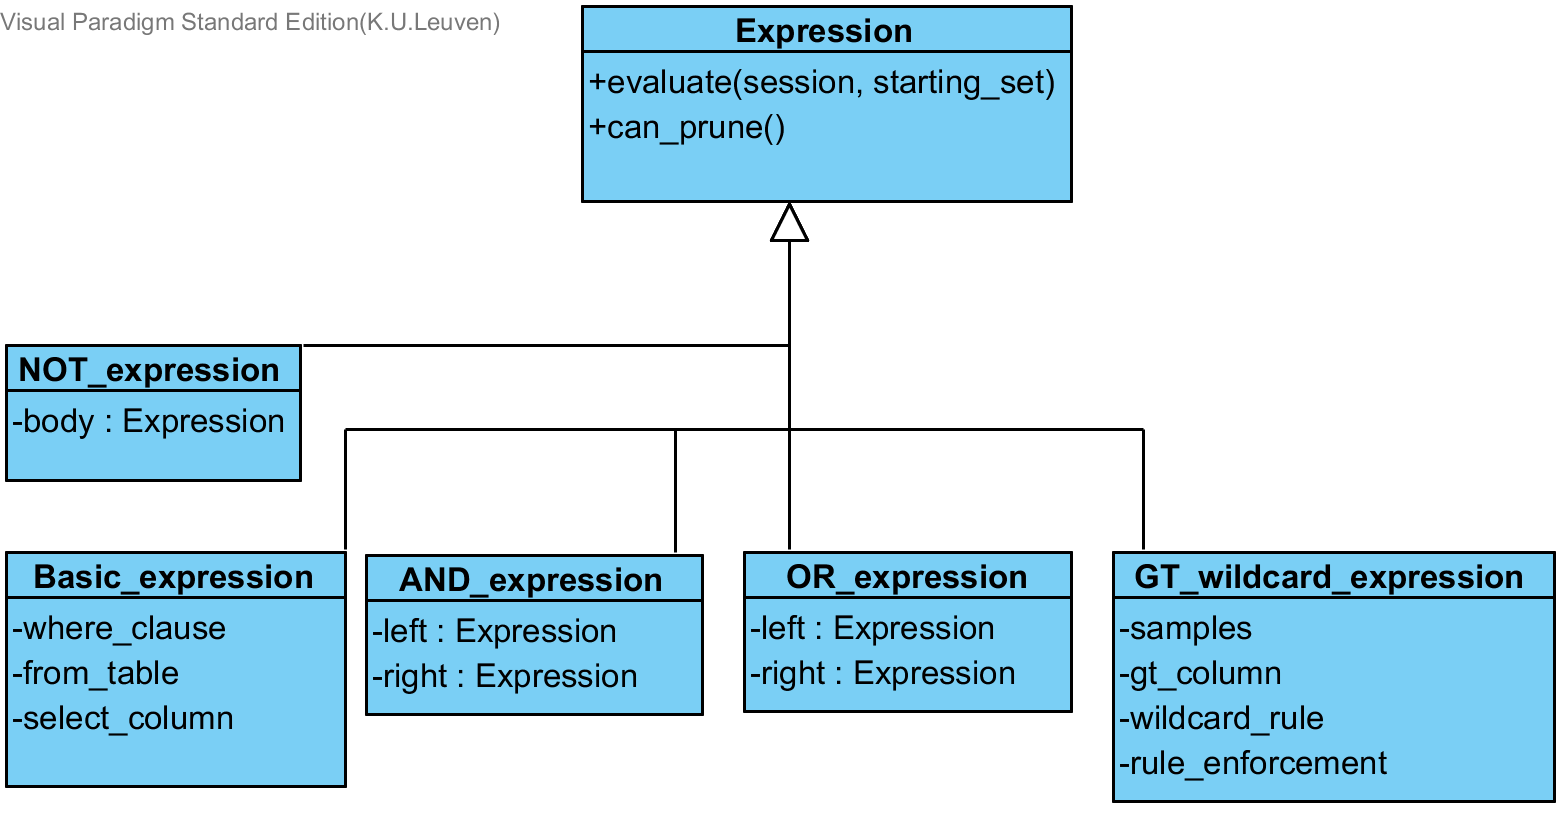
\includegraphics[width=\textwidth,height=\textheight,keepaspectratio]{query_exps}
\caption{De \texttt{query\_expressions} waarmee alle queries gemodelleerd worden. Het \texttt{session}-argument van de \texttt{evaluate}-functie is een actieve verbinding met het Cassandra-cluster.}
\label{query_exps_diagram}
\end{figure}

\subsubsection{Combineren subqueries}

Uit performantie-overwegingen is het een logische keuze de resultaten van subqueries op de hulptabellen te bewaren in een set datatype. Zo kunnen de benodigde set-operaties gebruik maken van de in Python ingebouwde set-operaties en zo veel effici\"enter verlopen dan wanneer de resultaten in bijvoorbeeld lists bewaard worden. Het enige nadeel van sets t.o.v. lists is dat de implementatie geen garanties biedt over in welke volgorde rijen in het eindresultaat zullen voorkomen. Dit weegt niet op tegen de tijdswinst, en bovendien biedt Cassandra zelf (in de algemeen aangeraden consistent hashing-partitionering) geen enkele garantie over in welke volgorde het rijen opslaat.\\\\
Bij het praktisch evalueren van \texttt{query\_expression}s komt uiteindelijk meer kijken dan enkel set-operaties. De belangrijkste reden hiervoor is dat, zoals in \ref{comb_subq_concept} reeds beschreven, om een negatie of \texttt{NOT\_expression} te kunnen evalueren, alle kandidaat-rijen gekend moet zijn, en dus meegegeven aan de \texttt{evaluate}-functie. Deze extra informatie kan ook bij het evalueren van andere types van \texttt{query\_expression} goed van pas komen.
 
\begin{itemize}
\item Het evalueren van \texttt{Basic\_expression}s gebeurt niet zo rechtoe rechtaan als de naam doet vermoeden. De \texttt{evaluate}-functie bouwt een CQL-query op, op basis van een gegeven \texttt{WHERE}-clausule, de relevante tabel en de gevraagde kolom uit die tabel. Wanneer er een zinvolle verzameling kandidaatrijen (de \texttt{starting\_set} in onderstaand codefragment) meegegeven is, wordt deze als \texttt{IN}-clausule aan de \texttt{WHERE}-clausule toegevoegd. Zo zoekt Cassandra enkel in rijen die effectief in aanmerking komen om aan de globale query te voldoen. Een voorwaarde om deze optimalisatie te kunnen toepassen, is dat de \texttt{WHERE}-clausule geen ongelijkheidsbeperkingen mag bevatten (vandaar de \texttt{can\_prune}-functie).

\lstinputlisting[language=Python,firstline=31,lastline=31]{gemini_src/query_expressions.py}
%TODO juist formatten, binnenste if, else verstoppen
\lstinputlisting[language=Python,firstline=36,lastline=53]{gemini_src/query_expressions.py}

\item Om een \texttt{AND\_expression} te evalueren is het strikt genomen nodig beide leden van de uitdrukking te evalueren en vervolgens de doorsnede te nemen van de resultaten. Als \'e\'en van de twee leden van de uitdrukking echter in staat is om dankzij een CQL \texttt{IN}-clausule enkel naar rijen te zoeken die effectief in aanmerking komen om aan de globale query te voldoen, is het mogelijk om deze operatie aan Cassandra over te laten. Als het rechterlid kan \textit{prunen}, dan kan GEMINI de resultaatverzameling van het linkerlid als \texttt{starting\_set} meegeven bij de evaluatie van het rechterlid, en omgekeerd. Wanneer geen van beide kunnen \textit{prunen}, moet GEMINI uiteraard nog steeds zelf de doorsnede berekenen.

\lstinputlisting[language=Python,firstline=64,lastline=64]{gemini_src/query_expressions.py}
\lstinputlisting[language=Python,firstline=69,lastline=77]{gemini_src/query_expressions.py}

\item In het geval van een \texttt{OR\_expression} is er geen andere mogelijkheid dan eenvoudigweg het linker- en rechterlid te evalueren, beide met als \texttt{starting\_set} de \texttt{starting\_set} van de \texttt{OR\_expression} zelf, en vervolgens de unie van de resultaten te berekenen.

\item Ook in het geval van een \texttt{NOT\_expression} is er geen andere optie dan de \texttt{body}-uitdrukking te evalueren en vervolgens het complement van de \texttt{starting\_set} en het resultaat te bepalen. Als de gegeven \texttt{starting\_set} gelijk is aan \texttt{"*"}, d.w.z. alle rijen in de oorspronkelijke tabel, zit er ook niets anders op dan deze nog eerst allemaal op te vragen.

\lstinputlisting[language=Python,firstline=112,lastline=112]{gemini_src/query_expressions.py}
\lstinputlisting[language=Python,firstline=116,lastline=123]{gemini_src/query_expressions.py}

\end{itemize}

Een optimalisatie die voor alle \texttt{query\_expressions} geldt is dat in het geval van een lege \texttt{starting\_set}, GEMINI de hele evaluatie kan overslaan. Dit bespaart een overtollige round-trip naar de Cassandra-databank. Voor alle soorten \texttt{query\_expressions} behalve \texttt{Basic\_expression} geldt ook dat ze kunnen \textit{prunen}, ongeacht de aard van hun subqueries. In het geval dat hun subqueries een \texttt{Basic\_expression} bevatten die niet kan \textit{prunen}, zal de subquery in kwestie dit zelf afhandelen bij de evaluatie.

\subsubsection{Genotype-filter wildcards}
\label{gt_wildcards}

Gegeven het bovenstaande query-mechanisme is de meest voor de hand liggende manier om genotype-filter wildcards te implementeren, deze op te splitsen in subqueries voor elke sample die aan de voorwaarden in de \texttt{sample\_wildcard} voldoet, en deze subqueries te combineren met een keten van geneste \texttt{query\_expression}s afhankelijk van de gegeven \texttt{rule\_enforcement}. Zo wordt een \texttt{all}-wildcard een keten van geneste \texttt{AND\_expression}s en een \texttt{any}-wildcard een keten van geneste \texttt{OR\_expression}s. \texttt{none}-wildcards vereisen eerst dat de subqueries in \texttt{NOT\_expression}d ingebed worden, die vervolgens allemaal in een keten van geneste \texttt{AND\_expression}s gecombineerd worden. Het is moeilijker \texttt{count}-wildcards tot dergelijke \texttt{expressions} om te vormen. Deze vergen een aparte strategie, die later aan bod komt.\\
Deze aanpak is vergelijkbaar met wat er in de SQLite- en PostgresQL-versies van GEMINI gebeurt: in SQLite vormt GEMINI de wildcards om tot lange Python-expressions die uiteindelijk voor elke variant met de Python \texttt{eval()}-functie ge\"evalueerd worden. Dit uiteraard omdat de genotype-kolommen bestaan uit binary blobs die voor de SQLite-databank geen enkele betekenis hebben. De PostgreSQL-versie van GEMINI pakt het slimmer aan en vormt de wildcards om tot lange SQL \texttt{WHERE}-clausules en laat zo het evaluatiewerk over aan de databank, met de bemerking dat de PostgreSQL-versie \texttt{count}-wildcards vooralsnog niet ondersteunt omdat dit niet rechtstreeks in SQL vertaald kunnen worden.\\
In dit opzicht lijkt de Cassandra-implementatie op de SQLite-implementatie, gezien de client, niet de databank, het meeste werk verricht.\\

Zoals in de conceptuele uitleg van de oplossing aangehaald, kan de evaluatie van genotype-wildcards effici\"enter verlopen door de evaluatie van de subqueries in parallel uit te voeren op meerdere processoren. Dit heb ik ook daadwerkelijk ge\"implementeerd, door introductie van een nieuw type \texttt{query\_expression}, namelijk de \texttt{GT\_wildcard\_expression}.\\
Bij evaluatie zal deze de namen van alle samples die aan de \texttt{sample\_wildcard} voldoen verdelen over het aantal processoren dat de gebruiker meegeeft, deze elk een tussenresultaat laten berekenen, de resultaten opvragen en samenvoegen m.b.v. de gekende setalgebra. Om het werk effici\"ent over verschillende processoren te verdelen en alle benodigde informatie te communiceren, maakt de implementatie gebruik van zogenaamde subprocesses, die elk hun eigen verbinding openen met het Cassandra-cluster, en interprocess-communicatiemechanismen uit de Python \texttt{multiprocessing}-API \cite{multiprocessing}.\\

\lstinputlisting[language=Python,firstline=186,lastline=210]{gemini_src/query_expressions.py}

\texttt{all-, any-} en \texttt{none-}wildcards vereisen voor het samenvoegen van de resultaten van de verschillende subprocesses geen grote aanpassingen aan de sequenti\"ele evaluatie-strategie van wildcards. Omdat deze oplossingswijze er zich uitstekend toe leent af te wijken van het stramien van de geneste \texttt{query\_expressions} (immers, er is maar 1 \texttt{GT\_wildcard\_expression} voor alle samples), is het makkelijker de \texttt{count}-wildcards te implementeren: elk subprocess voert subqueries uit voor de samples waarvoor het verantwoordelijk is en telt voor elke variant hoe vaak hij in de resultaatverzamelingen van de subqueries voorkomt. Deze informatie stuurt het subprocess terug naar zijn parent-process in een Python \textit{dictionary}, met een map van \texttt{variant\_id}s naar de telling.

\lstinputlisting[language=Python,firstline=328,lastline=357]{gemini_src/query_expressions.py}

Het parent-process kan vervolgens de telling voor alle variants van alle subprocesses bij elkaar optellen, en met gebruik van de Python \texttt{eval}-functie alle variants die aan de \texttt{count}-filter voldoen, bepalen. Let wel, bij het opstellen van de uiteindelijke \textit{dictionary} met de tellingen voor de varianten, moet het parent-process voor alle varianten in de \texttt{starting\_set}, een entry voorzien, met defaultwaarde 0. Zoniet zullen varianten waarvoor geen enkele sample aan de \texttt{gt\_wildcard\_rule} voldoet, niet in het resultaat voorkomen, en \texttt{count}-filters als \texttt{(count < x), (count <= x)} (voor arbitraire, positieve \texttt{x}) of \texttt{(count == 0)}  deze varianten onterecht niet in hun resultaat weergeven.

\lstinputlisting[language=Python,firstline=225,lastline=235]{gemini_src/query_expressions.py}

\noindent De \texttt{correct\_starting\_set} in bovenstaande code is de traditionele \texttt{starting\_set}, maar ge\"evalueerd in het geval dit de volledige verzameling varianten (dus de wildcard \texttt{"*"}) is, en gegoten in een datatype geschikt voor shared-memory access.\\
De \texttt{invert\_count}-flag geeft aan of de \texttt{gt\_wildcard\_rule} een negatie is. Gezien Cassandra geen \texttt{!=}-clausules ondersteunt, moet GEMINI in dit geval het complement van de \texttt{gt\_wildcard\_rule} in kwestie bepalen en vervolgens de resulterende telling aftrekken van het totaal aantal samples. \\ Een eenvoudig voorbeeld: bij het evalueren van volgende wildcard \\\\ 
\texttt{(gt\_type).(*).(!=HET).(count > 100)}\\\\
zal GEMINI eerst voor elke variant bepalen hoeveel samples w\'el heterozygoot zijn, alvorens dit getal af te trekken van het totaal aantal samples en op dit resultaat de \texttt{(count > 100)}-filter toe te passen.